% relatorio do t1: paralelizacao de path tracer smallpt com openmp
% a4, margem 1,5 cm, fonte 10, espacamento simples, no maximo 2 paginas
\documentclass[10pt,a4paper]{article}

\usepackage[utf8]{inputenc}
\usepackage[T1]{fontenc}
\usepackage[portuguese]{babel}
\usepackage[margin=1.5cm]{geometry}
\usepackage{multicol}
\usepackage{graphicx}
\usepackage{booktabs}
\usepackage{caption}
\usepackage{microtype}
\usepackage{amsmath}

\setlength{\columnsep}{0.5cm}
\setlength{\parskip}{1.5pt}
\setlength{\parindent}{0pt}
\setlength{\abovecaptionskip}{2pt}
\setlength{\belowcaptionskip}{0pt}
\captionsetup{font=footnotesize,labelfont=bf,skip=1pt}
\pagestyle{empty}
\makeatletter
\renewcommand\section{\@startsection{section}{1}{\z@}%
  {-0.55ex \@plus -0.1ex}{0.25ex}{\normalfont\normalsize\bfseries}}
\makeatother

\begin{document}

\begin{center}
  {\large\bfseries T1 -- Paraleliza\c{c}\~ao de uma aplica\c{c}\~ao com OpenMP}\\[1pt]
  {\small Computa\c{c}\~ao Paralela -- Unidade 03 \quad|\quad Aluno: Bernardo Klein Heitz}\\[0.5pt]
  {\footnotesize C\'odigo entregue em \texttt{.zip} junto deste PDF.}
\end{center}

\vspace{-6pt}
\begin{multicols}{2}
\raggedcolumns

\section*{1. O problema e o potencial de paraleliza\c{c}\~ao}
Paralelizamos com OpenMP um \emph{path tracer} no estilo \texttt{smallpt} de
Beason~\cite{beason2008}, reescrito em C11 (padr\~ao ISO C de 2011). O programa
integra a ilumin\^ancia de uma Cornell Box de nove esferas (paredes difusas,
uma especular e uma refrativa) por amostragem de Monte Carlo, com $2\times 2$
subpixels e roleta russa a partir da profundidade 5. A entrada
\texttt{-w 800 -h 600 -s 32} coloca o sequencial em $T_1\approx 54$\,s: h\'a um
la\c{c}o externo independente por linha, os materiais impedem um
\texttt{parallel for} trivial, e $w$, $h$ e $\mathrm{spp}$ parametrizam o
trabalho.

A escolha do eixo veio do \texttt{gprof} na mesma entrada e na mesma fase do
speed-up (bin\'ario \texttt{-O2 -fno-inline -pg}). \texttt{radiance} e as
rotinas que ela chama somam $98{,}2\%$ do tempo; \texttt{main} fica com
$1{,}75\%$. A fra\c{c}\~ao paraleliz\'avel \'e $f\approx 0{,}982$, logo
$S_{\max}(6)=1/(0{,}018+0{,}982/6)\approx 5{,}51$,
$S_{\max}(12)\approx 10{,}00$ e $S_{\infty}=1/(1-f)\approx 55{,}6$. No bin\'ario
\texttt{-O3} de medi\c{c}\~ao, $\mathtt{time\_par\_s}/\mathtt{time\_s}=0{,}99998$:
a parcela serial da fase medida \'e desprez\'ivel. O $7{,}44\times$ da
Se\c{c}\~ao~5 fica abaixo de $S_{\max}(12)$, portanto a satura\c{c}\~ao n\~ao se
deve a essa fra\c{c}\~ao.

\section*{2. Ambiente e metodologia}
CPU AMD Ryzen 5 3600 (6 n\'ucleos f\'isicos, 12 processadores l\'ogicos,
$3{,}6$\,GHz base), L3 de $32$\,MB, $32$\,GB de RAM DDR4. SO Ubuntu 22.04 em
WSL2 sobre Windows 11. Compilador \texttt{gcc 11.4.0}, flags id\^enticas
\texttt{-O3 -march=native -ffast-math -std=c11}; a vers\~ao paralela acrescenta
s\'o \texttt{-fopenmp}. $T_1$ vem do bin\'ario compilado sem \texttt{-fopenmp},
n\~ao da vers\~ao OpenMP com uma thread. \texttt{omp\_get\_num\_procs()} devolve
12. Medimos com \texttt{omp\_get\_wtime()} a fase computacional completa
(c\^amera, aloca\c{c}\~ao, la\c{c}o e checksum); escrita PPM e print CSV ficam
fora, nos dois bin\'arios. Cada ponto teve 10 execu\c{c}\~oes em m\'aquina
ociosa; reportamos mediana, m\'inimo e m\'aximo. Threads fixadas por
\texttt{OMP\_NUM\_THREADS}. O checksum RGB \'e id\^entico de 1 a 12 threads e em
todas as pol\'iticas.

\section*{3. Modelagem e diretivas}
A unidade de trabalho \'e uma linha da imagem ($600$ itera\c{c}\~oes em
\texttt{y}). As linhas n\~ao s\~ao homog\^eneas: as que cruzam o espelho e o
vidro ricocheteiam mais; as do fundo preto terminam cedo. O perfil com
\texttt{nowait} mesmo assim mostra desvio entre threads abaixo de $1\%$; o que
pesa \'e a preemp\c{c}\~ao do WSL2, n\~ao a cena. Cada itera\c{c}\~ao escreve
numa faixa disjunta de \texttt{c}, o que dispensa \texttt{atomic},
\texttt{critical} e \texttt{reduction} no caminho quente. Um gerador global
exigiria \texttt{critical} em cada \texttt{rng\_next} e serializaria dezenas de
milh\~oes de chamadas. O xorshift64 ficou local ao corpo do la\c{c}o, com
semente derivada de \texttt{y}, e o checksum deixou de depender do n\'umero de
threads.

Os pragmas est\~ao em \texttt{src/smallpt.c:320--332}:
\texttt{\#pragma omp parallel default(none) shared(...)} envolve
\texttt{\#pragma omp for schedule(runtime) nowait} sobre o la\c{c}o em
\texttt{y}. O \texttt{default(none)} obriga listar o escopo. O buffer
\texttt{c} tem escrita disjunta; \texttt{stat} \'e indexado por
\texttt{omp\_get\_thread\_num()} com padding de $64$\,B contra falso
compartilhamento. \texttt{schedule(runtime)} troca a pol\'itica por
\texttt{OMP\_SCHEDULE}; \texttt{nowait} faz o tempo por thread refletir a
carga real, n\~ao a barreira.

\section*{4. Balanceamento de carga}
Testamos sete pol\'iticas em 12 threads, 10 execu\c{c}\~oes cada
(Tabela~\ref{tab:sched}). \texttt{dynamic,4} teve a menor mediana
($7{,}16$\,s) e a menor dispers\~ao ($7{,}01$ a $7{,}35$\,s).
\texttt{static} sem chunk ficou em \'ultimo ($9{,}56$\,s; $7{,}57$ a
$11{,}78$\,s), embora o desvio interno seja inferior a $1\%$. A
heterogeneidade das linhas n\~ao explica esse gap: no WSL2 uma thread
preemptada no \texttt{static} segura o bloco inteiro, enquanto
\texttt{dynamic,4} redistribui peda\c{c}os de quatro linhas. Adotamos
\texttt{dynamic,4} por essa medi\c{c}\~ao, nas duas escalabilidades.

\section*{5. An\'alise dos resultados}
A Figura~\ref{fig:speedup} e a Tabela~\ref{tab:strong} descrevem a
escalabilidade forte (entrada fixa). At\'e 6 threads o speed-up acompanha
Amdahl: $4{,}93$ medidos contra o teto $5{,}51$, efici\^encia $82{,}2\%$. O
afastamento j\'a vis\'ivel em 4 threads ($3{,}31$ contra o teto $3{,}73$) n\~ao
\'e fra\c{c}\~ao sequencial -- essa parcela \'e $<0{,}002\%$ da fase medida --,
e sim o custo de criar o time OpenMP e a disputa por L3. No ponto em que o SMT
entra (linha vertical em 6 threads nas Figuras~\ref{fig:speedup}
e~\ref{fig:eff}) a curva se dobra. De 6 para 8 o speed-up vai a $6{,}14$
($+25\%$) e a efici\^encia cai a $76{,}8\%$; de 10 para 12 o ganho adicional \'e
$1{,}8\%$ e a efici\^encia cai a $62{,}0\%$. O \texttt{smallpt} \'e limitado por
ponto flutuante em \texttt{double}: duas threads no mesmo n\'ucleo competem
pelas unidades FP e pela cache. O $7{,}44\times$ em 12 threads fica abaixo de
$S_{\max}(12)\approx 10$, logo a satura\c{c}\~ao \'e SMT somado \`a
preemp\c{c}\~ao do WSL2, n\~ao \`a fra\c{c}\~ao sequencial.

\end{multicols}

\vspace{-6pt}
\begin{minipage}[t]{0.49\textwidth}
\centering
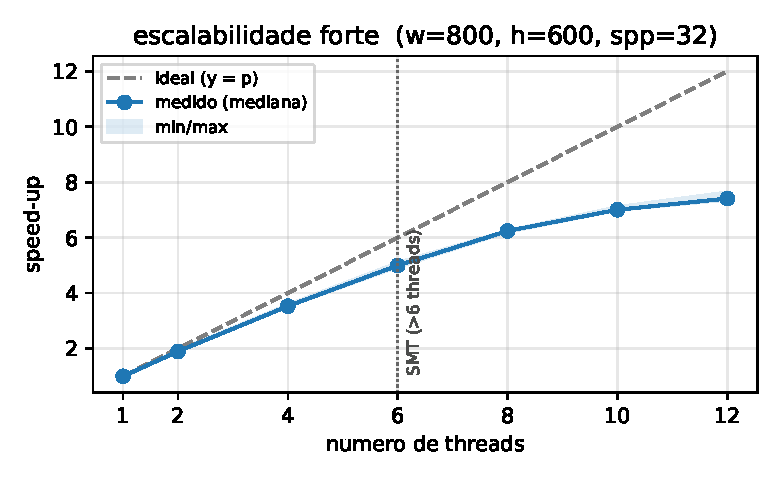
\includegraphics[height=3.15cm,keepaspectratio]{../results/speedup.pdf}
\captionof{figure}{Speed-up da escalabilidade forte (mediana de 10
  execu\c{c}\~oes) contra $y=p$. A faixa \'e o min--max. A linha em 6 threads
  marca o in\'icio do SMT.}
\label{fig:speedup}
\end{minipage}\hfill
\begin{minipage}[t]{0.49\textwidth}
\centering
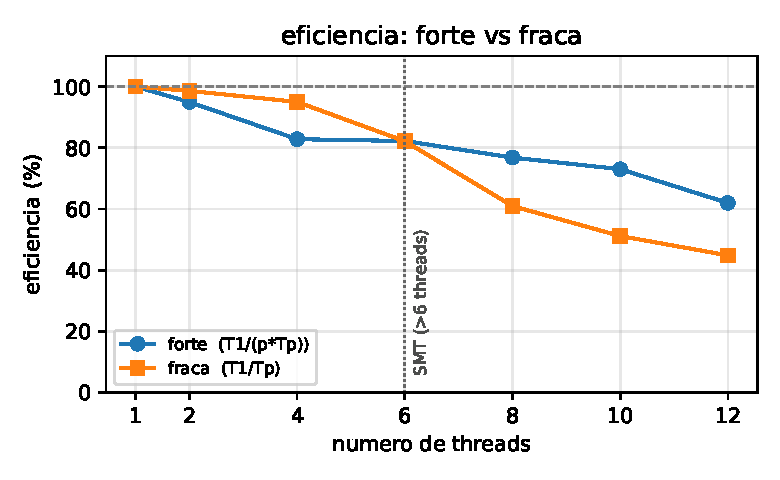
\includegraphics[height=3.15cm,keepaspectratio]{../results/efficiency.pdf}
\captionof{figure}{Efici\^encia forte ($T_1/(p\,T_p)$) e fraca ($T_1/T_p$).
  Ambas quebram no SMT; a fraca cai mais a partir de 8 threads.}
\label{fig:eff}
\end{minipage}

\vspace{2pt}
A escalabilidade fraca (Figura~\ref{fig:eff}, Tabela~\ref{tab:weak}) parte da
mesma entrada e escala $\mathrm{spp}=32\cdot p$, porque o custo \'e
$O(w\cdot h\cdot\mathrm{spp})$: o trabalho total cresce com $p$ e o trabalho
por thread permanece aproximadamente constante. At\'e 4 threads o tempo quase
n\~ao sobe ($55{,}6$, $56{,}4$ e $58{,}6$\,s; efici\^encia $\ge 95\%$), o que
\'e o comportamento esperado de uma aplica\c{c}\~ao sem fra\c{c}\~ao serial
vis\'ivel. Em 6 threads vai a $67{,}7$\,s ($82{,}2\%$, igual \`a da forte): o
primeiro n\'ucleo extra ainda cabe na topologia f\'isica. Passado o SMT a fraca
piora mais: $91{,}3$\,s em 8 threads e $124{,}1$\,s em 12 ($44{,}8\%$ contra
$62{,}0\%$ da forte). Com trabalho por thread constante, 12 threads em 6
n\'ucleos colocam duas cargas completas no mesmo n\'ucleo; o tempo esperado
seria $2\times 67{,}7\approx 135$\,s e medimos $124$\,s -- o SMT recupera cerca
de $8\%$. Na forte o trabalho total \'e fixo, ent\~ao o SMT ainda reduz
$10{,}9$\,s para $7{,}3$\,s. As duas curvas quebram no mesmo ponto: a causa \'e
a topologia da m\'aquina, n\~ao o algoritmo nem Amdahl.

A dispers\~ao das 10 repeti\c{c}\~oes aponta para o mesmo s\'itio. Na forte, o
intervalo min--max cresce de $0{,}3$\,s em 2 threads para $1{,}4$\,s em 12. Na
fraca explode em 6 e 8 threads ($60{,}6$ a $73{,}5$\,s e $76{,}4$ a
$102{,}6$\,s) e fecha de novo em 12 ($123{,}3$ a $125{,}6$\,s). Corridas longas
no WSL2 convivem com o host Windows: o \texttt{dynamic,4} mascara a thread
preemptada, mas o tempo de parede sobe. Em 12 threads a m\'aquina j\'a est\'a
saturada, a interfer\^encia relativa cai e a dispers\~ao diminui. O $T_1$ da
fraca ($55{,}6$\,s) difere do da forte ($54{,}0$\,s) porque as campanhas foram
em momentos distintos; usamos o $T_1$ de cada campanha. A diferen\c{c}a de
$3\%$ \'e ru\'ido de m\'aquina. Em resumo, at\'e os 6 n\'ucleos f\'isicos o
path tracer escala perto do teto de Amdahl; al\'em disso o SMT da
microarquitetura Zen~2 n\~ao oferece unidades FP extras, e a fraca -- que
mant\'em trabalho por thread -- denuncia isso com mais clareza que a forte.

\vspace{1pt}
{\footnotesize Um assistente de IA revisou o arn\^es de medi\c{c}\~ao, o script
de plotagem e a estrutura deste relat\'orio. Cada decis\~ao de c\'odigo
(escopo, \texttt{dynamic,4}, rng por linha, \texttt{nowait}) foi conferida com
as medi\c{c}\~oes acima.}

\vspace{-6pt}
\begin{thebibliography}{1}
\bibitem{beason2008}
K.~Beason.
\newblock \emph{smallpt: global illumination in 99 lines of C++}, 2008.
\end{thebibliography}

\vspace{-8pt}
\setlength{\tabcolsep}{4.2pt}
\begin{center}
\footnotesize
\captionof{table}{Escalabilidade forte ($w{=}800$, $h{=}600$, $\mathrm{spp}{=}32$),
  10 execu\c{c}\~oes. $T_1$ \'e o sequencial sem \texttt{-fopenmp}.}
\label{tab:strong}
\begin{tabular}{r r r r r r}
  \toprule
  Threads & Med.\ (s) & Min (s) & Max (s) & Speed-up & Ef. \\
  \midrule
  1 ($T_1$) & 53{,}996 & 53{,}552 & 56{,}206 & 1{,}000 & 100{,}0\% \\
  2  & 28{,}437 & 28{,}126 & 30{,}418 & 1{,}899 & 94{,}9\% \\
  4  & 16{,}300 & 15{,}307 & 16{,}929 & 3{,}313 & 82{,}8\% \\
  6  & 10{,}945 & 10{,}512 & 12{,}057 & 4{,}933 & 82{,}2\% \\
  8  &  8{,}789 &  8{,}349 &  9{,}032 & 6{,}144 & 76{,}8\% \\
  10 &  7{,}395 &  6{,}991 &  7{,}672 & 7{,}302 & 73{,}0\% \\
  12 &  7{,}261 &  6{,}456 &  7{,}846 & 7{,}437 & 62{,}0\% \\
  \bottomrule
\end{tabular}

\vspace{5pt}
\captionof{table}{Escalabilidade fraca. Regra $\mathrm{spp}=32\cdot p$
  (custo linear em spp). Efici\^encia $=T_1/T_p$.}
\label{tab:weak}
\begin{tabular}{r r r r r r}
  \toprule
  Threads & spp & Med.\ (s) & Min (s) & Max (s) & Ef. \\
  \midrule
  1 ($T_1$) &  32 & 55{,}643 & 54{,}551 & 57{,}554 & 100{,}0\% \\
  2  &  64 & 56{,}432 & 55{,}605 & 59{,}526 & 98{,}6\% \\
  4  & 128 & 58{,}578 & 57{,}927 & 59{,}572 & 95{,}0\% \\
  6  & 192 & 67{,}730 & 60{,}617 & 73{,}468 & 82{,}2\% \\
  8  & 256 & 91{,}290 & 76{,}362 & 102{,}594 & 61{,}0\% \\
  10 & 320 & 108{,}754 & 107{,}091 & 110{,}528 & 51{,}2\% \\
  12 & 384 & 124{,}098 & 123{,}328 & 125{,}584 & 44{,}8\% \\
  \bottomrule
\end{tabular}

\vspace{5pt}
\captionof{table}{Pol\'iticas de escalonamento em 12 threads, 10 execu\c{c}\~oes,
  mesma entrada da forte.}
\label{tab:sched}
\begin{tabular}{l r r r}
  \toprule
  Pol\'itica & Mediana (s) & Min (s) & Max (s) \\
  \midrule
  static               & 9{,}556 & 7{,}573 & 11{,}779 \\
  static, 32           & 8{,}389 & 7{,}425 & 10{,}494 \\
  static, 4            & 7{,}658 & 7{,}259 &  8{,}287 \\
  dynamic              & 7{,}297 & 7{,}210 &  7{,}933 \\
  dynamic, 32          & 7{,}199 & 7{,}157 &  7{,}608 \\
  dynamic, 4 (adotada) & 7{,}164 & 7{,}006 &  7{,}354 \\
  guided               & 7{,}231 & 6{,}935 &  7{,}385 \\
  \bottomrule
\end{tabular}
\end{center}

\end{document}
